\documentclass[12pt,letterpaper]{article}
\usepackage[utf8]{inputenc}
\usepackage[spanish]{babel}
\usepackage{graphicx}
\usepackage[left=2cm,right=2cm,top=2cm,bottom=2cm]{geometry}
\usepackage{graphicx} % figuras
% \usepackage{subfigure} % subfiguras
\usepackage{float} % para usar [H]
\usepackage{amsmath}
%\usepackage{txfonts}
\usepackage{stackrel} 
\usepackage{multirow}
\usepackage{enumerate} % enumerados
\renewcommand{\labelitemi}{$-$}
\renewcommand{\labelitemii}{$\cdot$}
% \author{}
% \title{Caratula}
\begin{document}

% Fancy Header and Footer
% \usepackage{fancyhdr}
% \pagestyle{fancy}
% \cfoot{}
% \rfoot{\thepage}
%

% \usepackage[hidelinks]{hyperref} % CREA HYPERVINCULOS EN INDICE

% \author{}
\title{Caratula}

\begin{titlepage}
\begin{center}
\large{UNIVERSIDAD PRIVADA DE TACNA}\\
\vspace*{-0.025in}
\begin{figure}[htb]
\begin{center}

\includegraphics[width=8cm]{./Imagenes/logo}
\end{center}
\end{figure}
\vspace*{0.15in}
INGENIERIA DE SISTEMAS  \\

\vspace*{0.5in}
\begin{large}
TITULO:\\
\end{large}

\vspace*{0.1in}
\begin{Large}
\textbf{Informe Laboratorio Nro 05 Inteligencia de Negocios} \\
\end{Large}

\vspace*{0.3in}
\begin{Large}
\textbf{CURSO:} \\
\end{Large}

\vspace*{0.1in}
\begin{large}
INTELIGENCIA DE NEGOCIOS\\
\end{large}

\vspace*{0.3in}
\begin{Large}
\textbf{DOCENTE(ING):} \\
\end{Large}

\vspace*{0.1in}
\begin{large}
 Patrick Cuadros Quiroga\\
\end{large}

\vspace*{0.2in}
\vspace*{0.1in}
\begin{large}
Integrantes: \\
\begin{flushleft}
Perez Mamani Nilton Edy		 \hfill	(2015053233) \\
\end{flushleft}
\end{large}
\end{center}

\end{titlepage}


\tableofcontents % INDICE
\thispagestyle{empty} % INDICE SIN NUMERO
\newpage
\setcounter{page}{1} % REINICIAR CONTADOR DE PAGINAS DESPUES DEL INDICE

\begin{document}
PRACTICA 1: IMPORTACION, DATA FLOW, TRASLADO DE ARCHIVOS
\section{Objetivos}
✓ IMPORTAR DATOS USANDO EL WIZARD Y Desarrollar mis primeros PAQUETEs DTSX

\section{Requerimientos}

✓ “REQUERIMIENTOS: SQL SERVER INTEGRATION SERVICES 2012R2, BD ADVENTURE WORK (OLTP Y DATAWAREHOUSE) y AdventureWorksLT2012”
\\

\section{IMPORTACION DE DATOS USANDO EL WIZARD – SQL MANAGMENT}
\item{
\textbf{Crear una base de datos – BDTEST}
\begin{center}
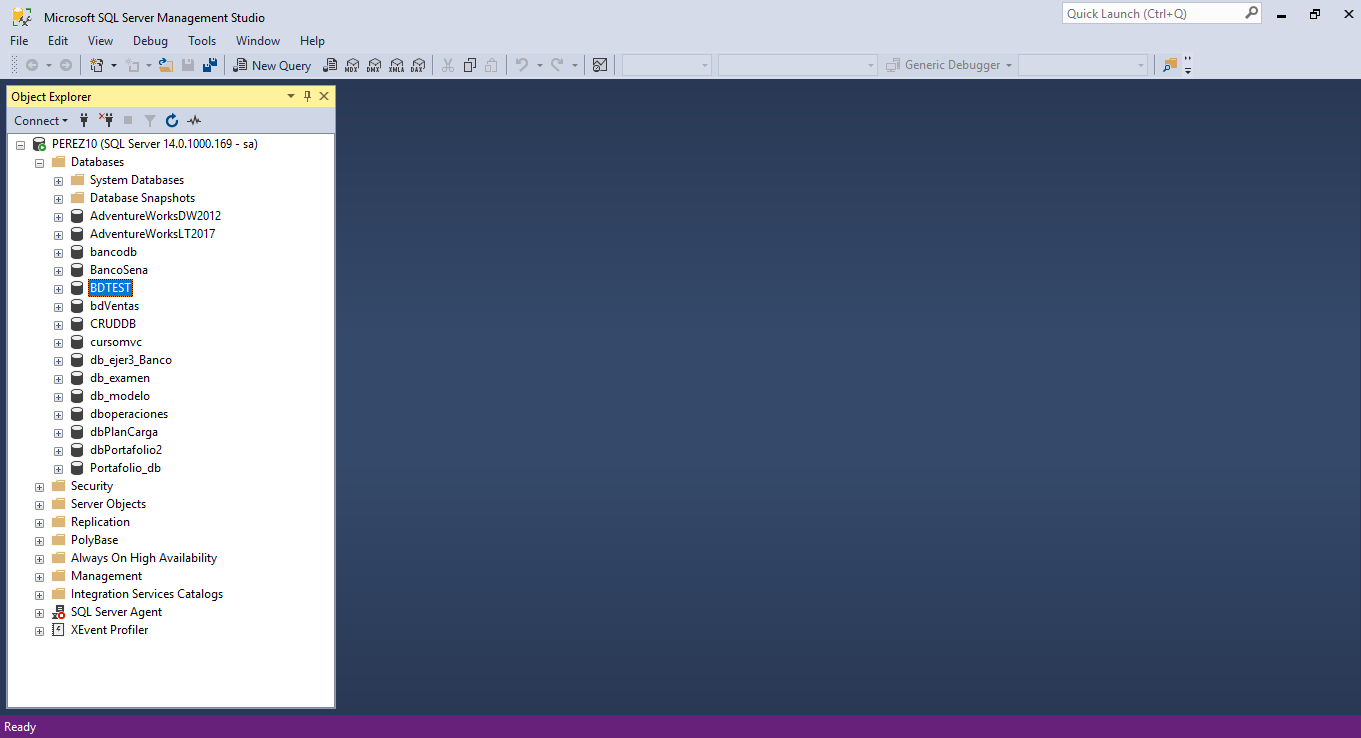
\includegraphics[width=15cm]{./Imagenes/imagen1}
\end{center}
\textbf{Importar Datos desde AdventureWorks}
\begin{center}
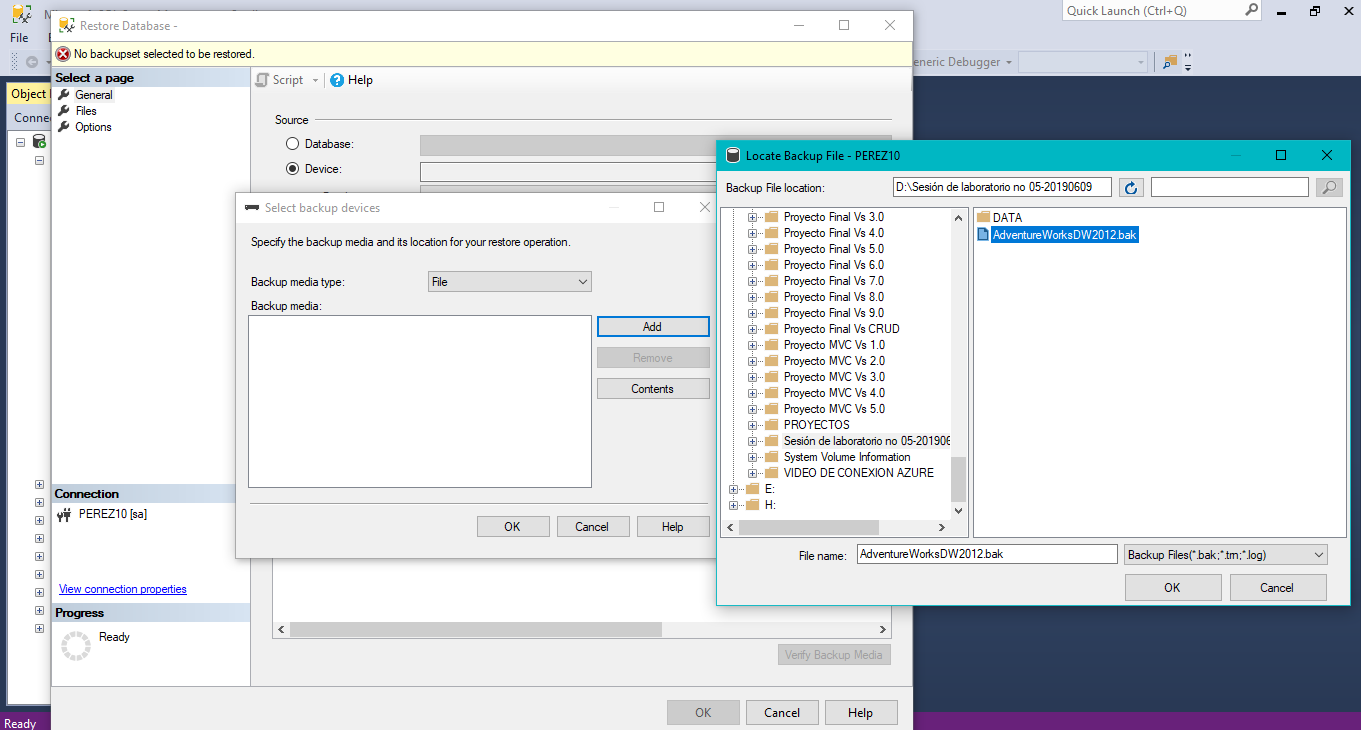
\includegraphics[width=15cm]{./Imagenes/imagen2}
\end{center}
\textbf{Next y escribir el Servidor y seleccionar la base de datos}
\begin{center}
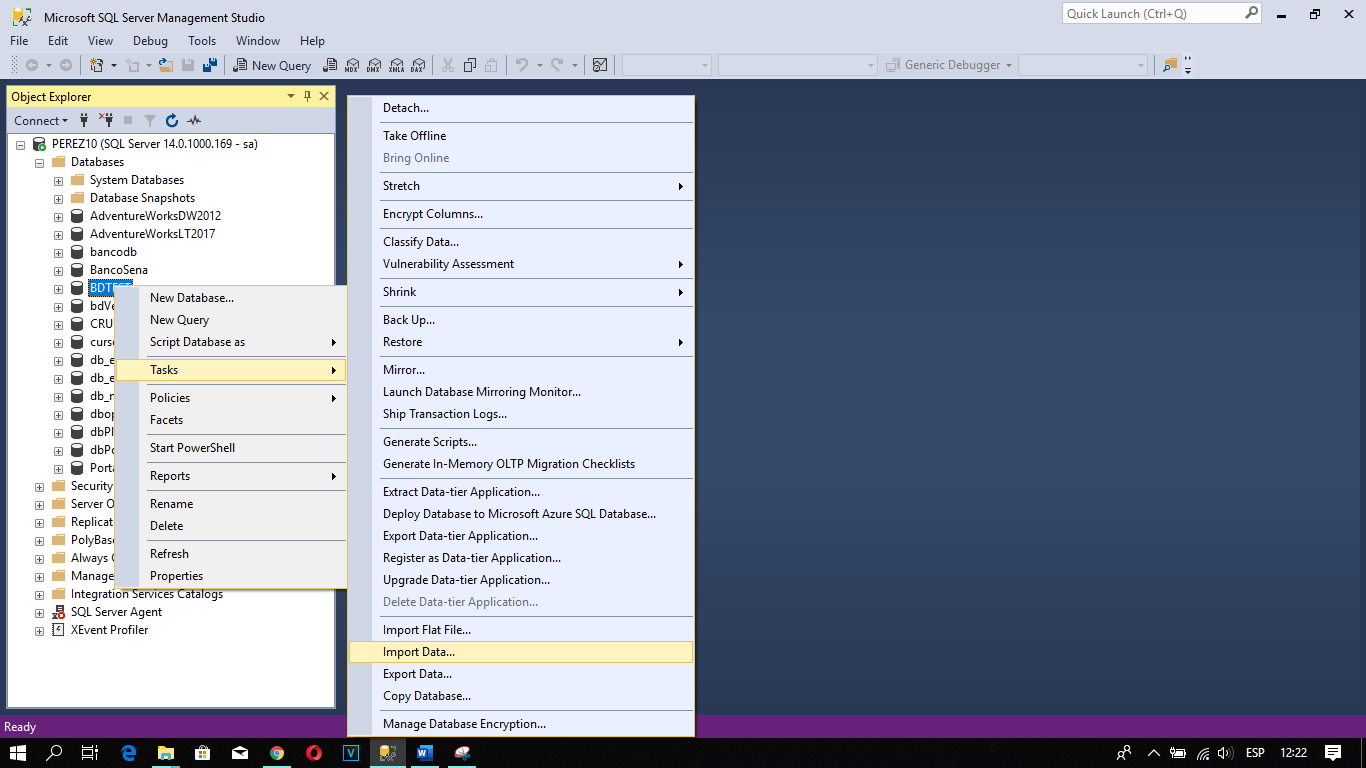
\includegraphics[width=15cm]{./Imagenes/imagen3}
\end{center}
\begin{center}
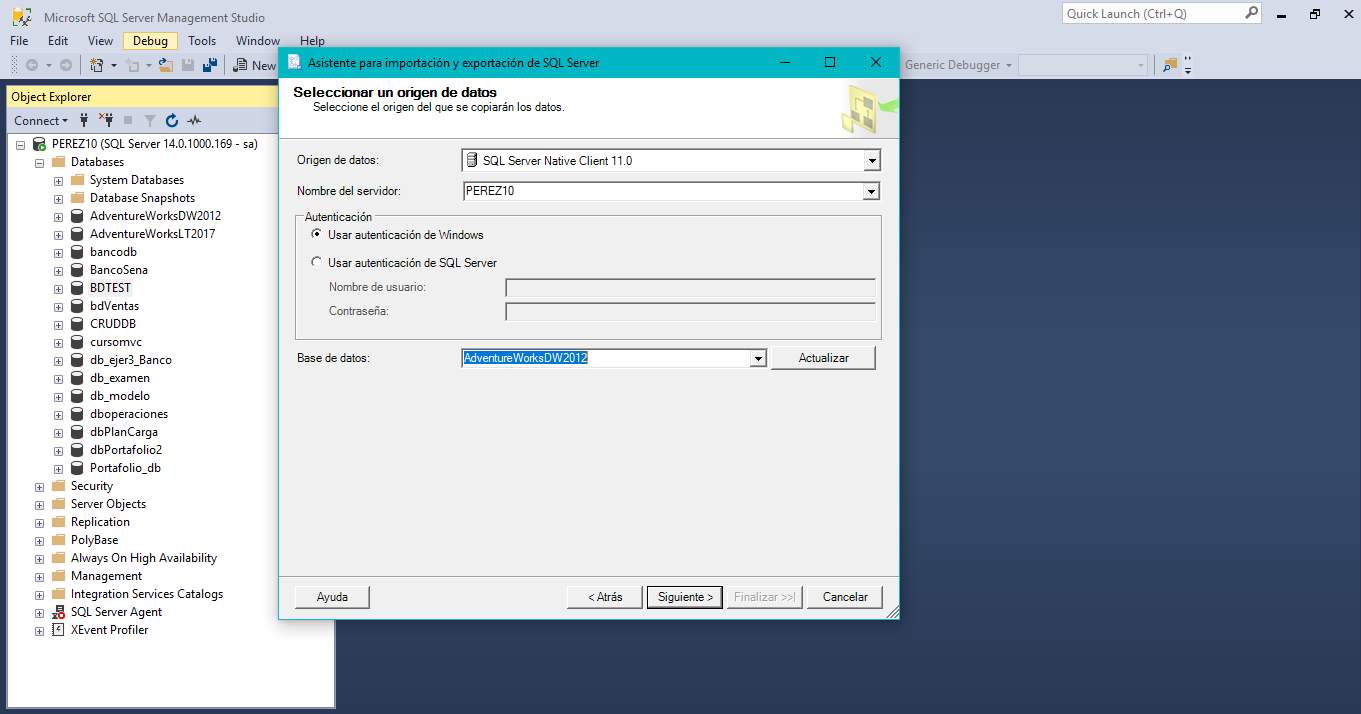
\includegraphics[width=15cm]{./Imagenes/imagen4}
\end{center}
\begin{center}
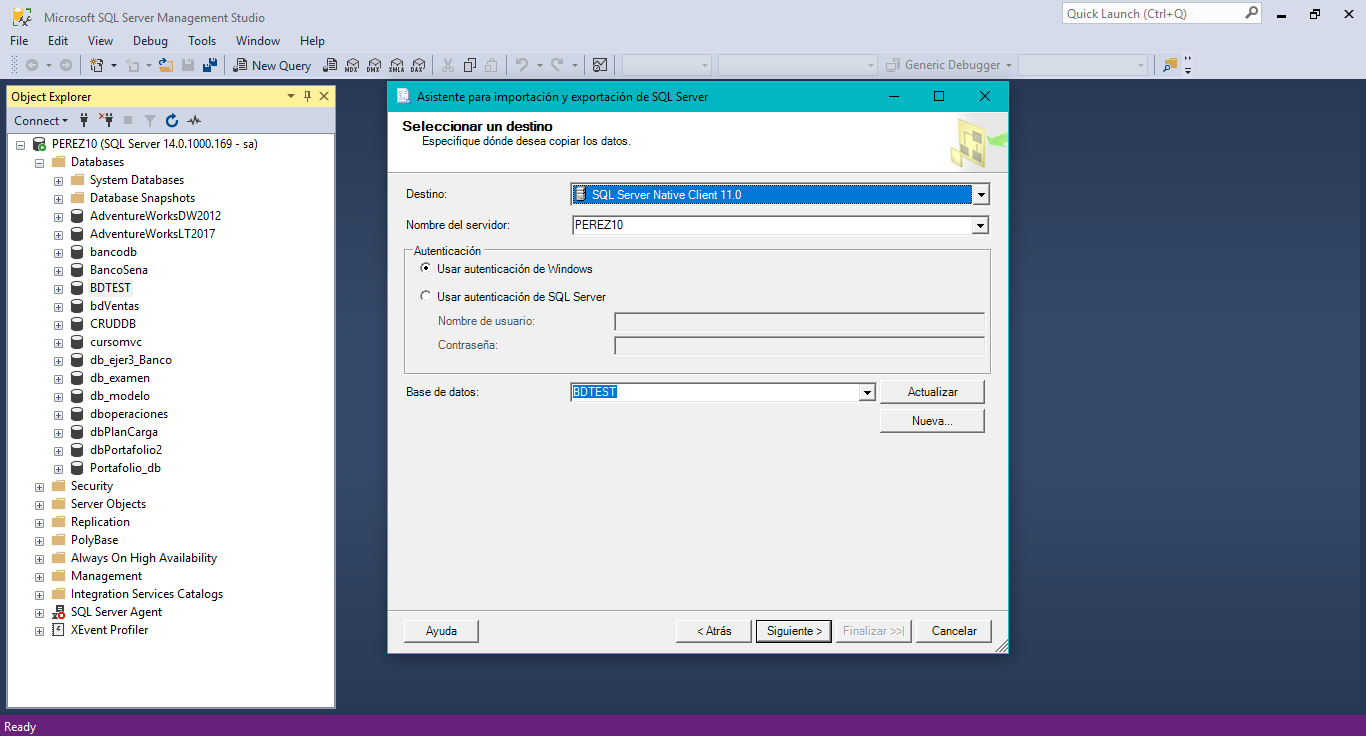
\includegraphics[width=15cm]{./Imagenes/imagen5}
\end{center}
\begin{center}
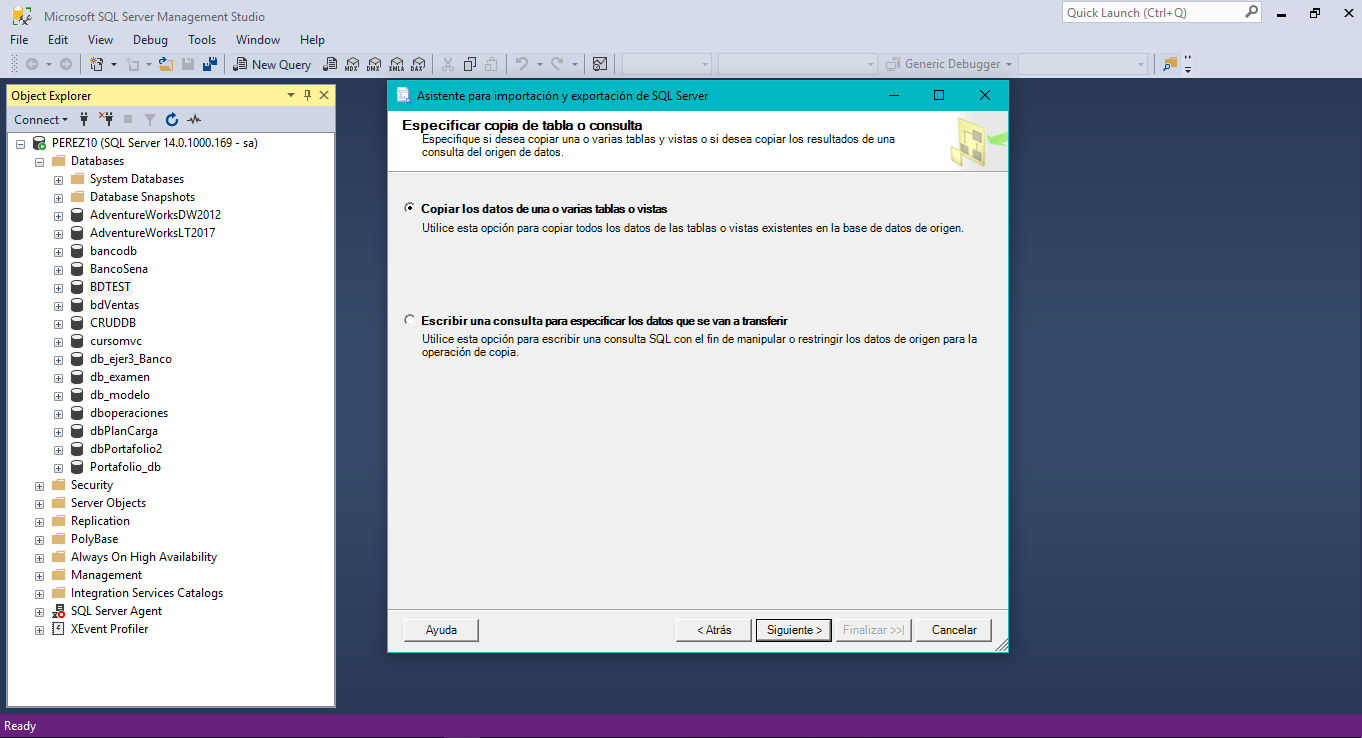
\includegraphics[width=15cm]{./Imagenes/imagen6}
\end{center}
\begin{center}
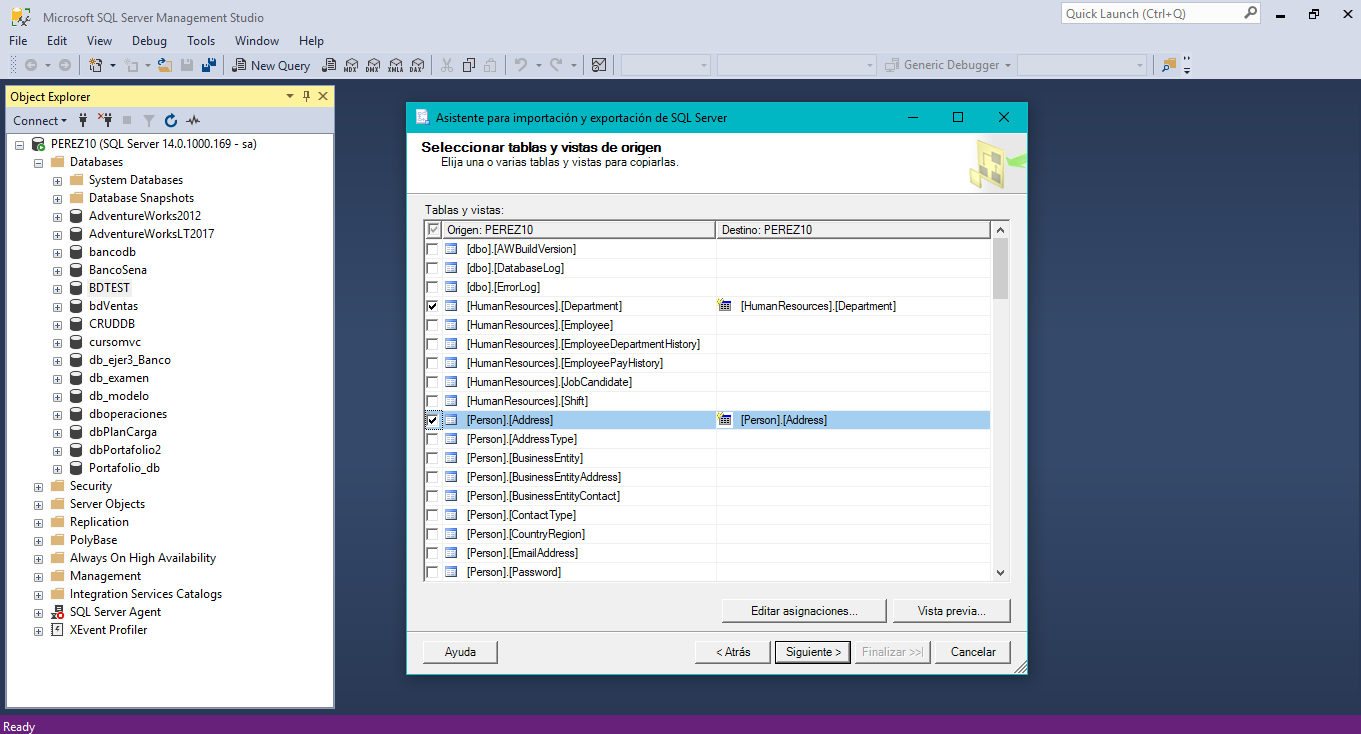
\includegraphics[width=15cm]{./Imagenes/imagen7}
\end{center}
\begin{center}
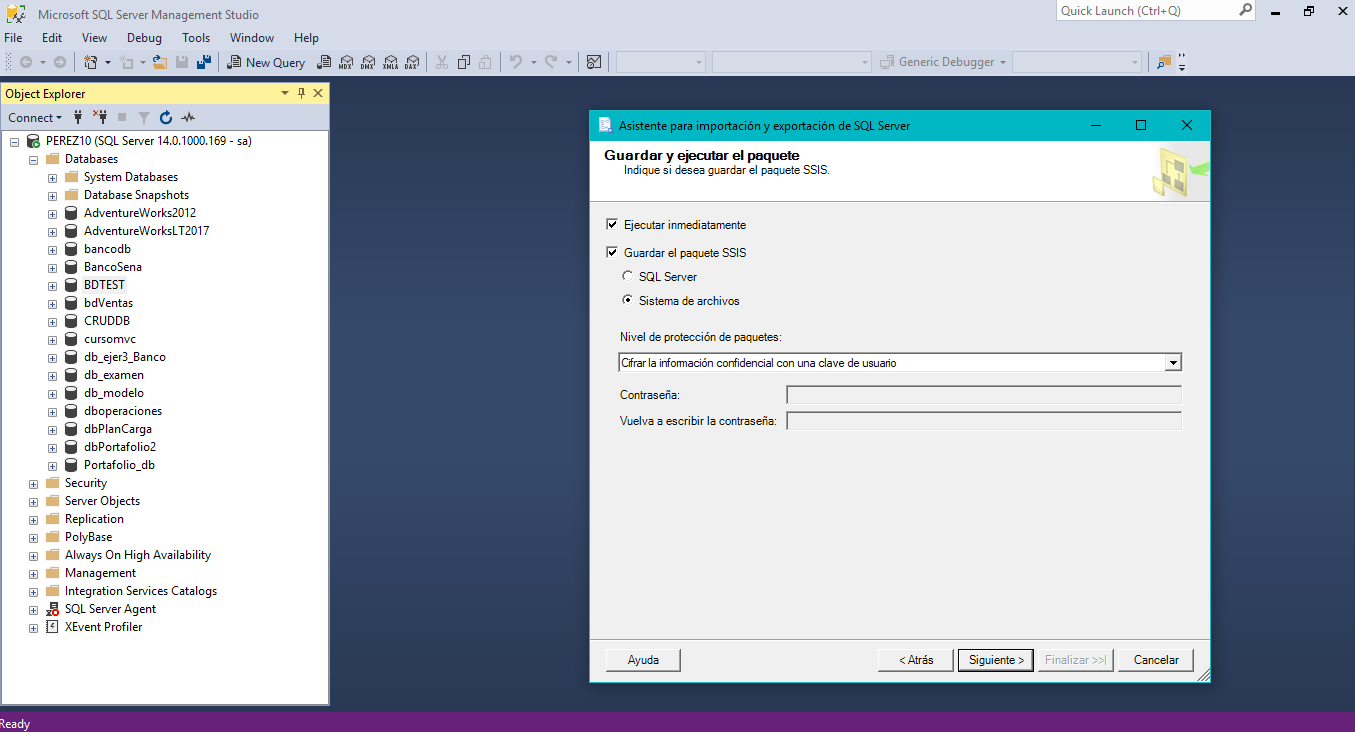
\includegraphics[width=15cm]{./Imagenes/imagen8}
\end{center}
\begin{center}
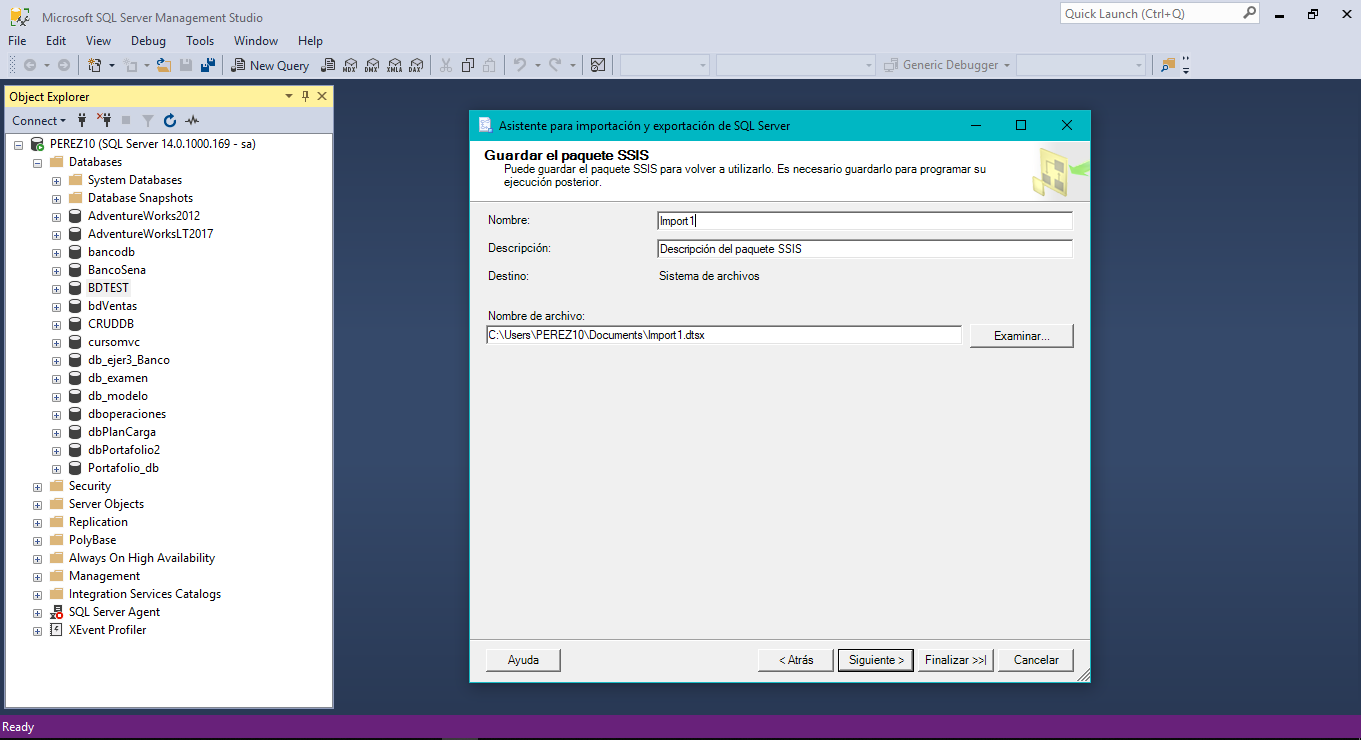
\includegraphics[width=15cm]{./Imagenes/imagen9}
\end{center}
\begin{center}
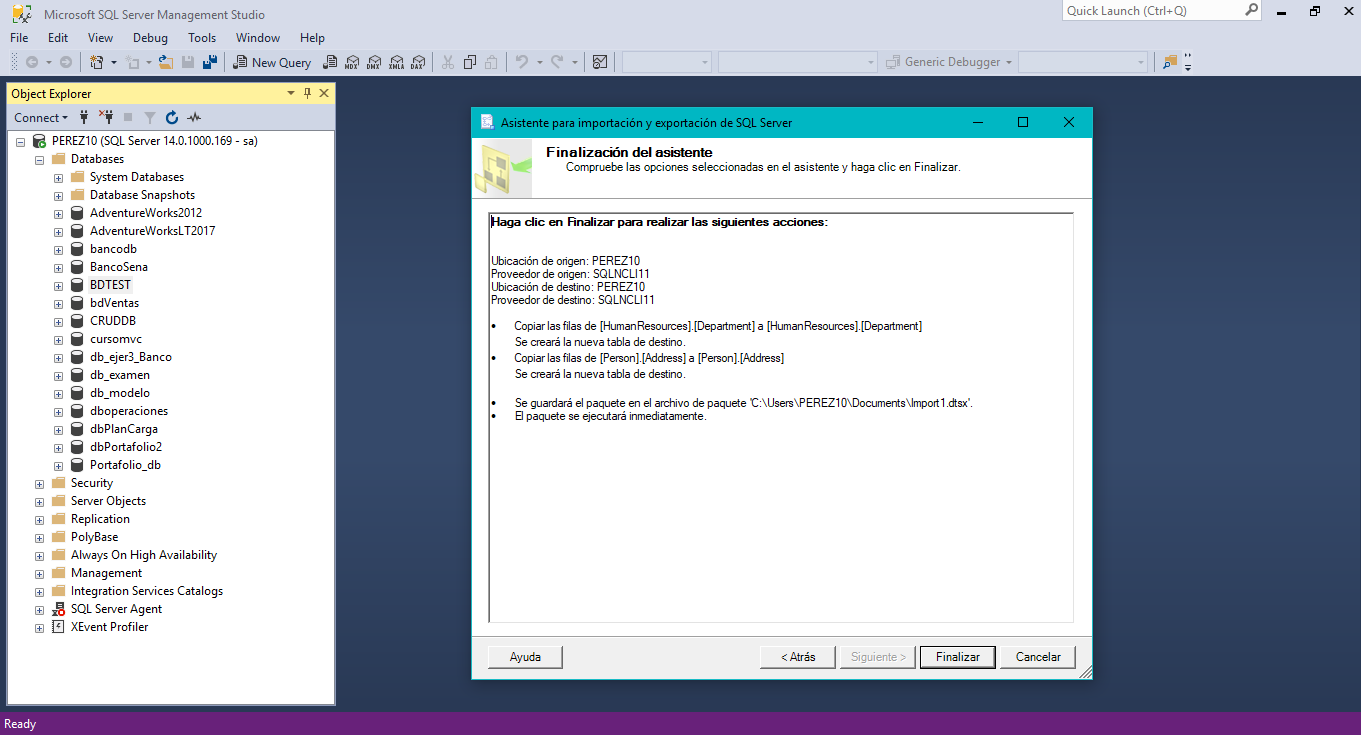
\includegraphics[width=15cm]{./Imagenes/imagen10}
\end{center}
\begin{center}
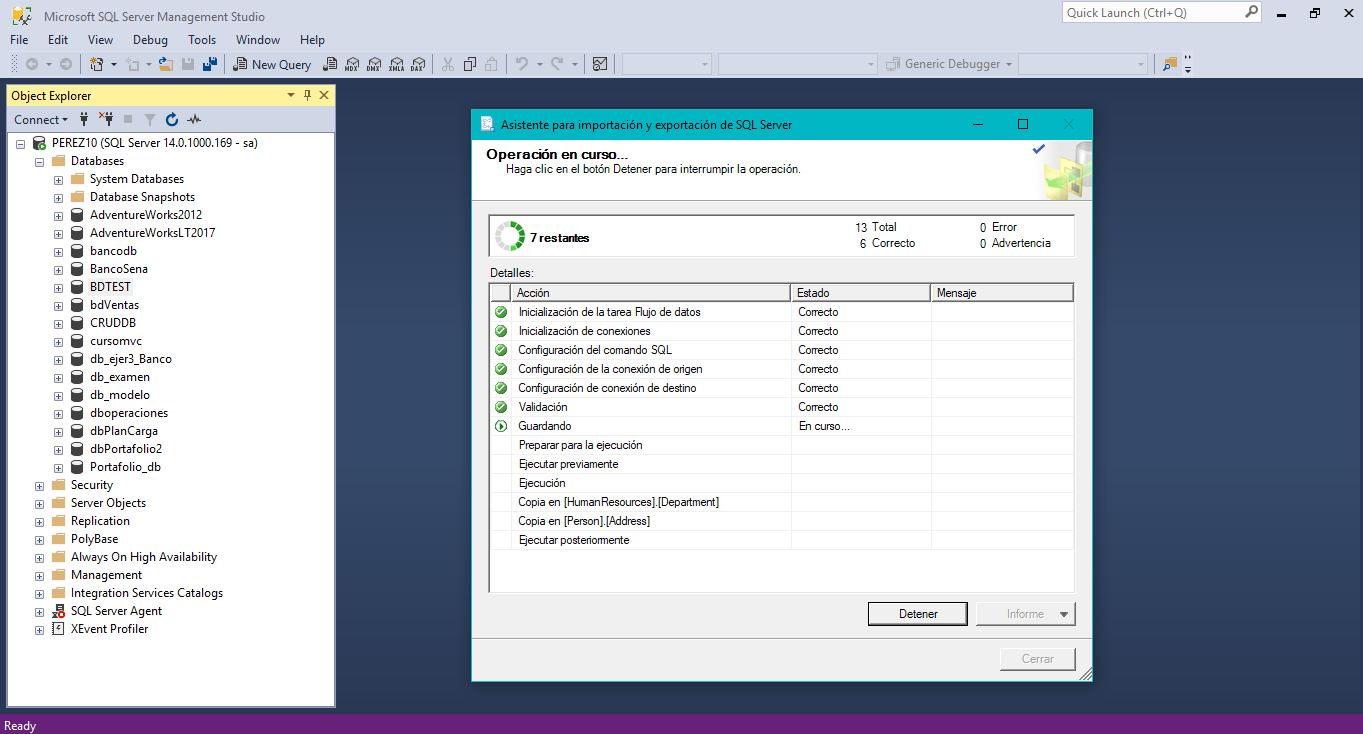
\includegraphics[width=15cm]{./Imagenes/imagen11}
\end{center}
\begin{center}
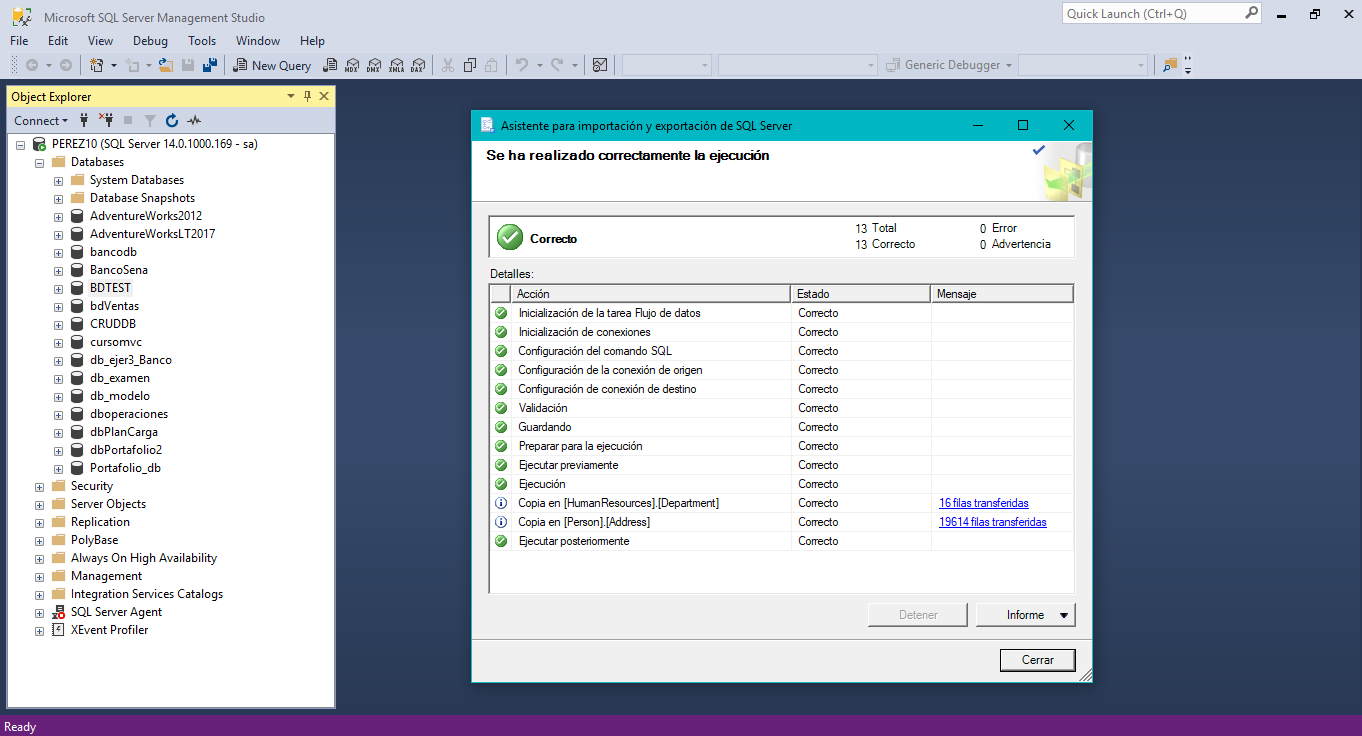
\includegraphics[width=15cm]{./Imagenes/imagen12}
\end{center}
}

\section{CREAMOS NUESTRO PRIMER PAQUETE DTSX}
\item{
\begin{center}
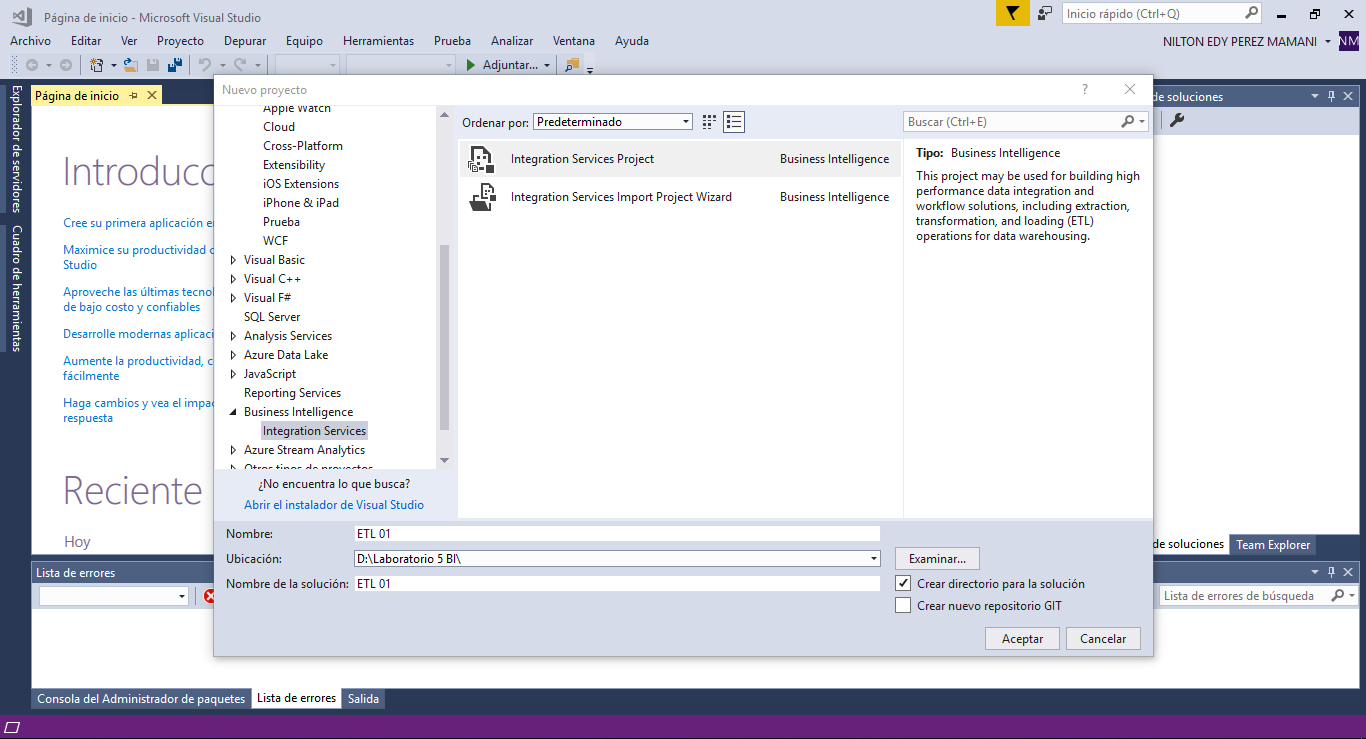
\includegraphics[width=15cm]{./Imagenes/imagen13}
\end{center}
\begin{center}
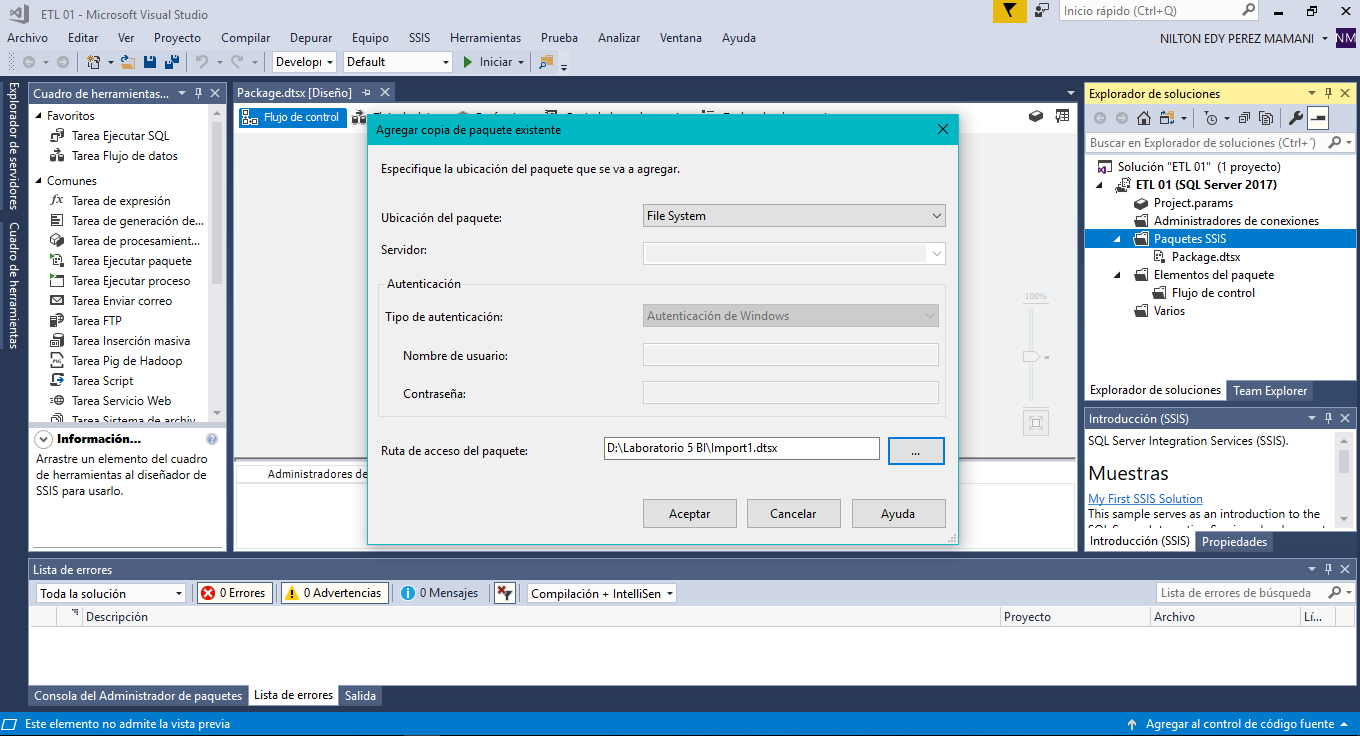
\includegraphics[width=15cm]{./Imagenes/imagen14}
\end{center}
\begin{center}
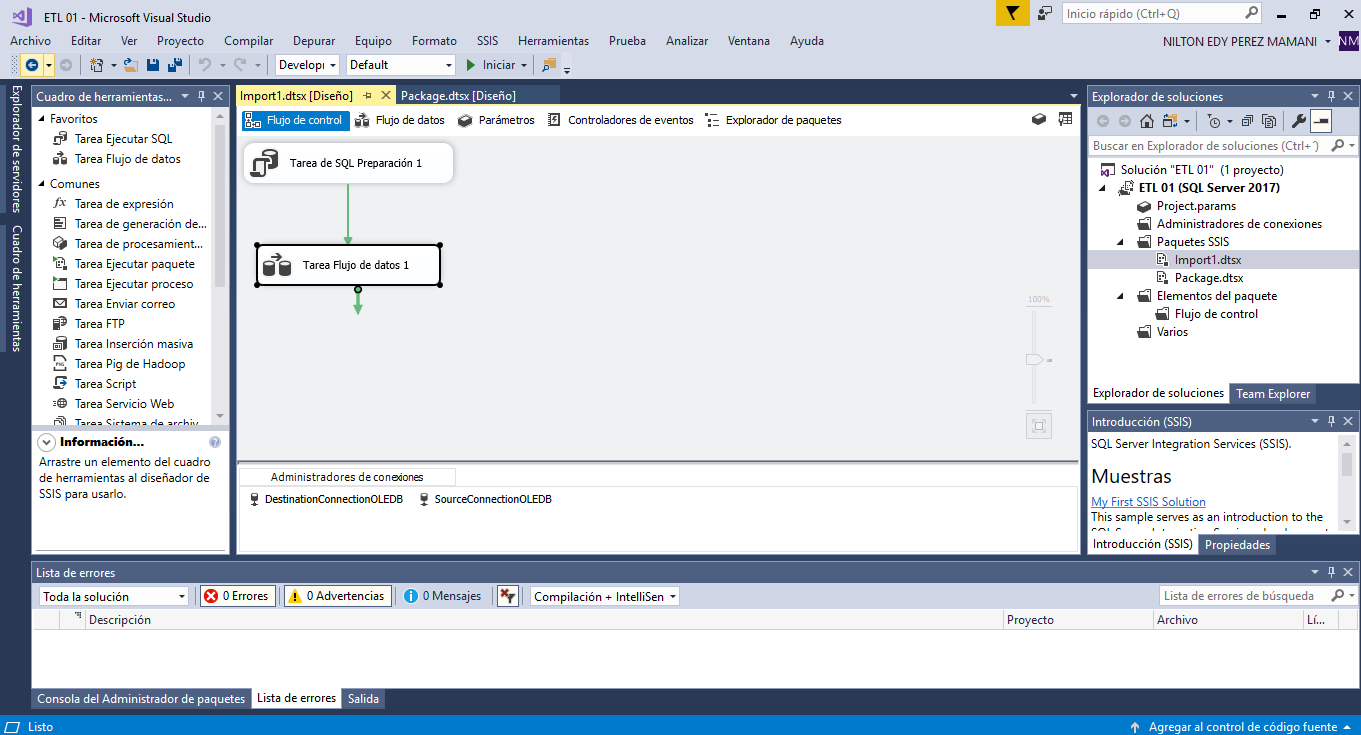
\includegraphics[width=15cm]{./Imagenes/imagen15}
\end{center}
\begin{center}
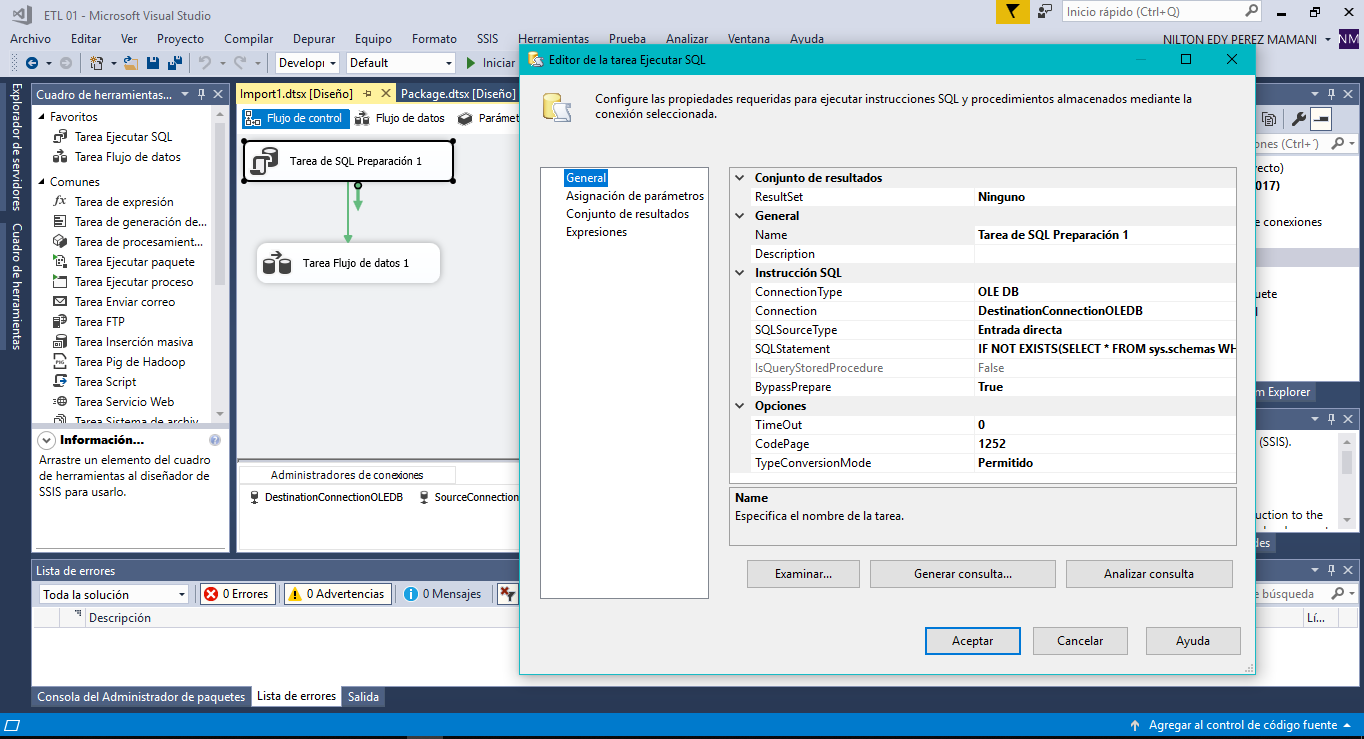
\includegraphics[width=15cm]{./Imagenes/imagen16}
\end{center}
\begin{center}
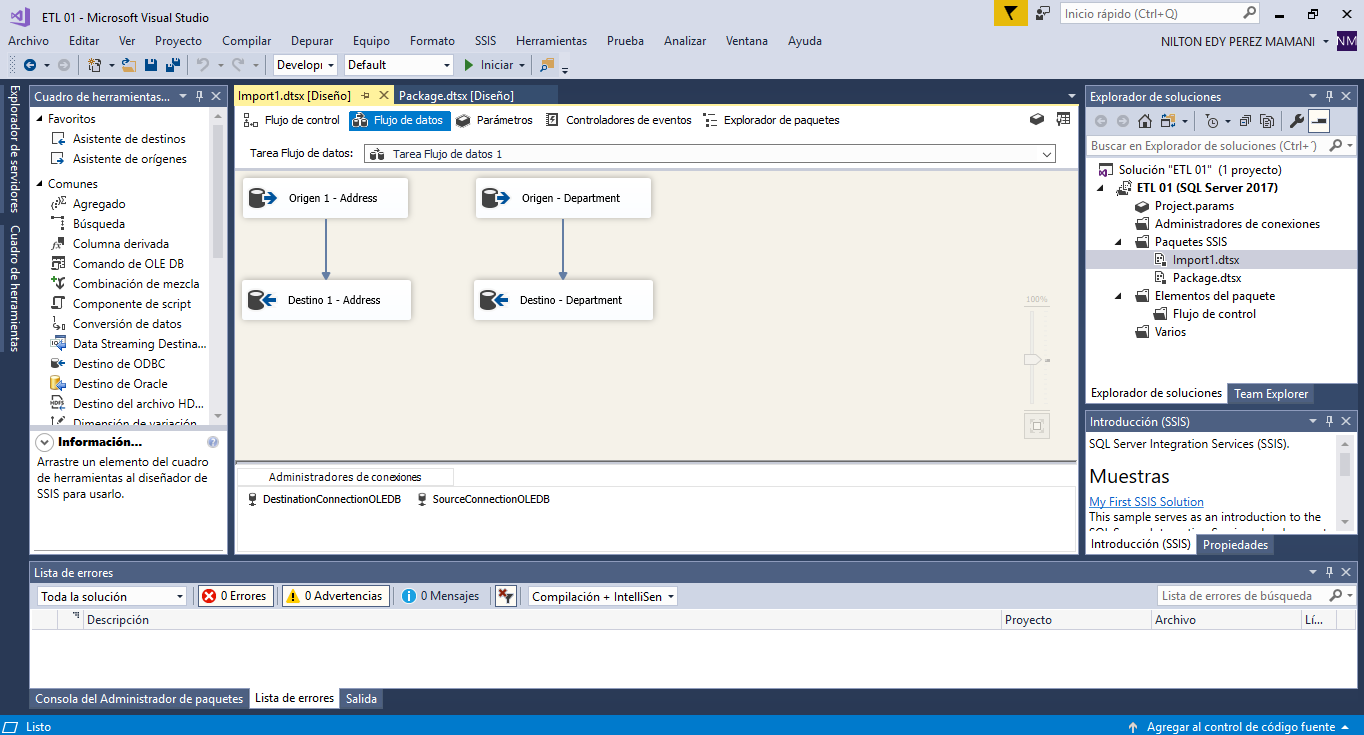
\includegraphics[width=15cm]{./Imagenes/imagen17}
\end{center}
\begin{center}
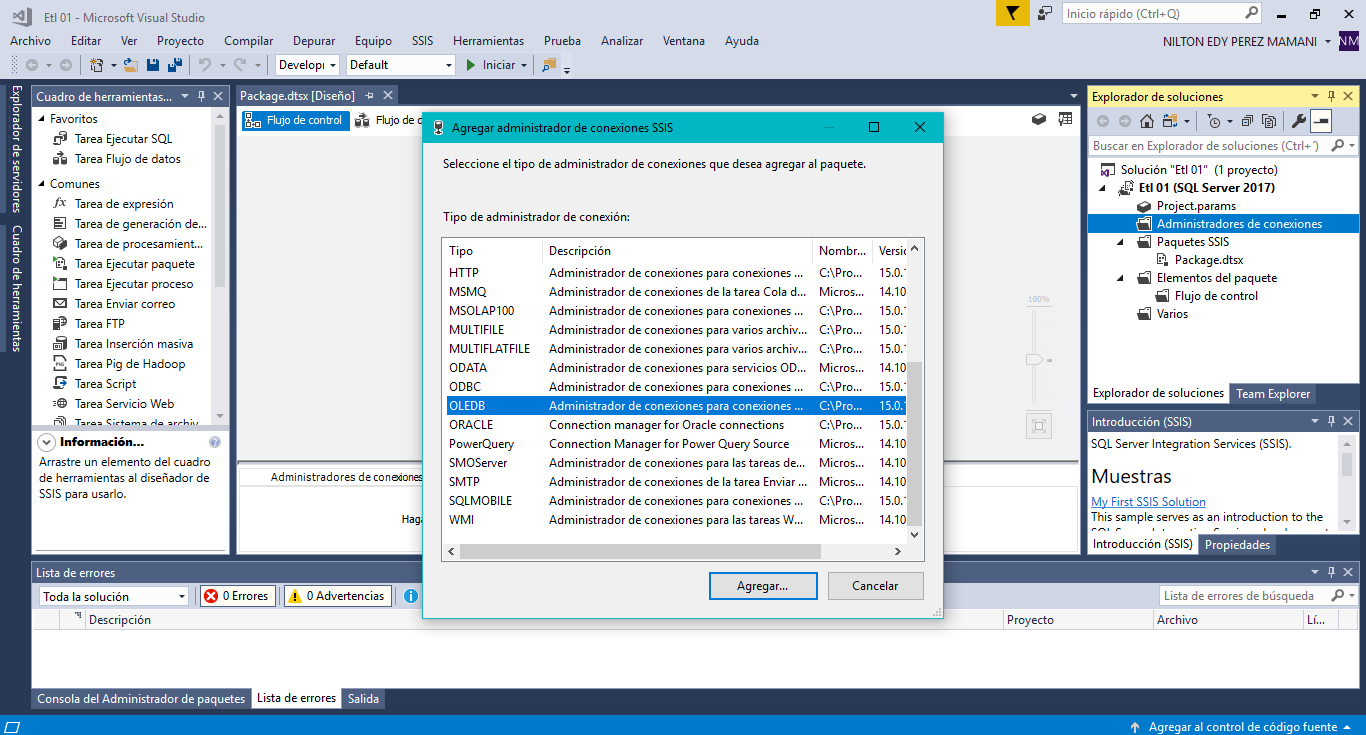
\includegraphics[width=15cm]{./Imagenes/imagen18}
\end{center}
\begin{center}
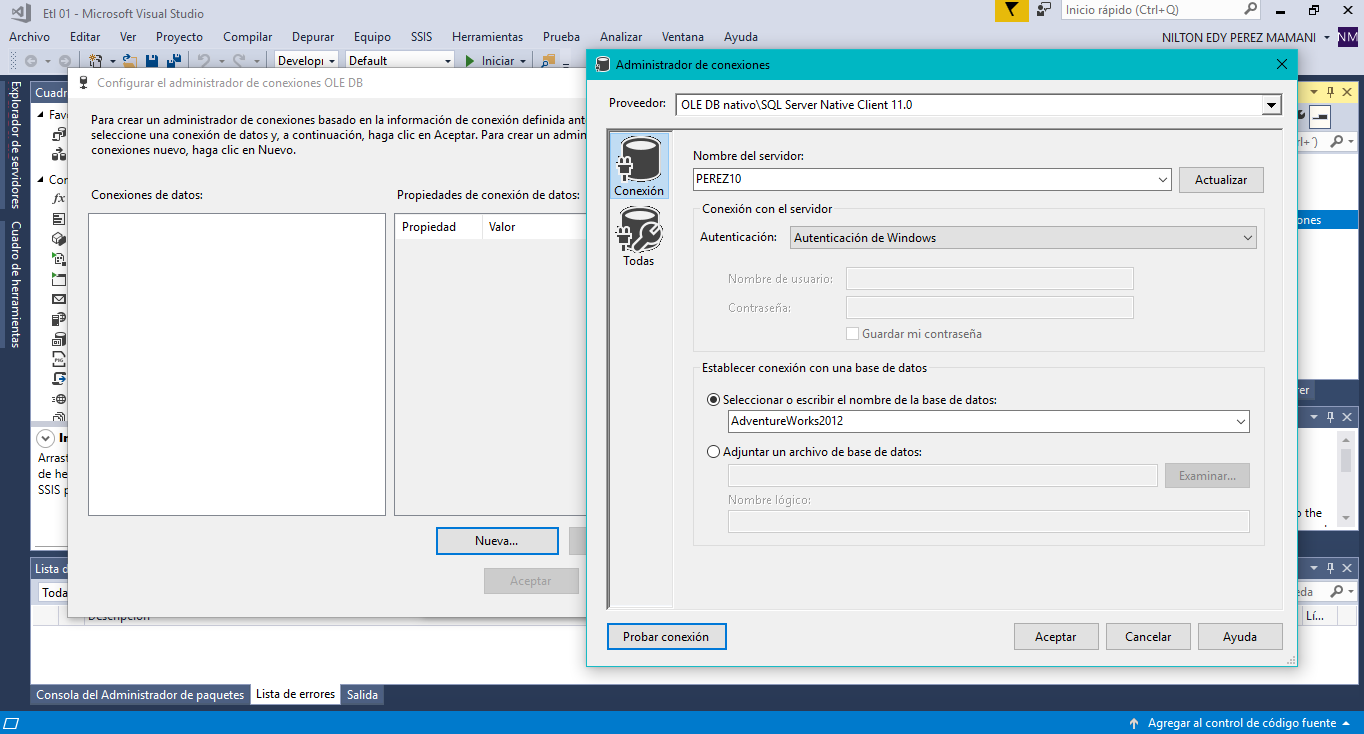
\includegraphics[width=15cm]{./Imagenes/imagen19}
\end{center}
\begin{center}
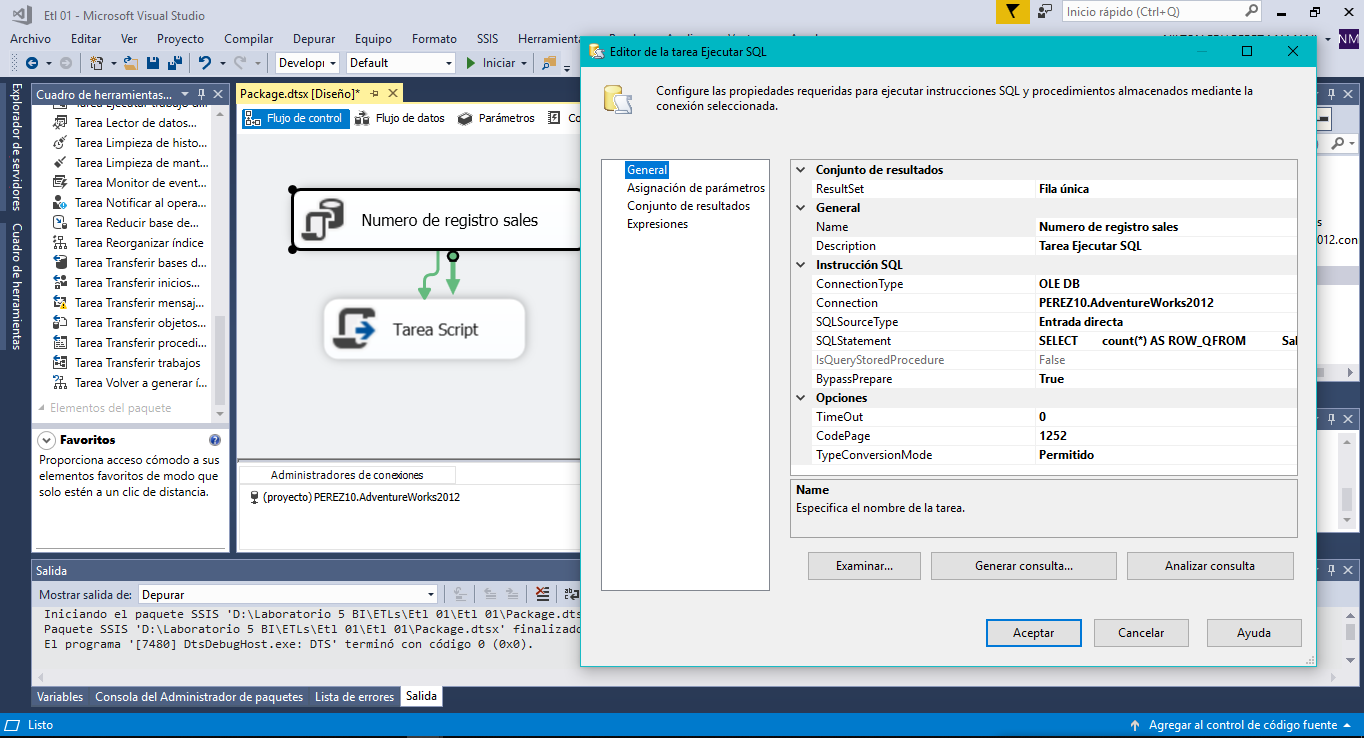
\includegraphics[width=15cm]{./Imagenes/imagen20}
\end{center}
\begin{center}
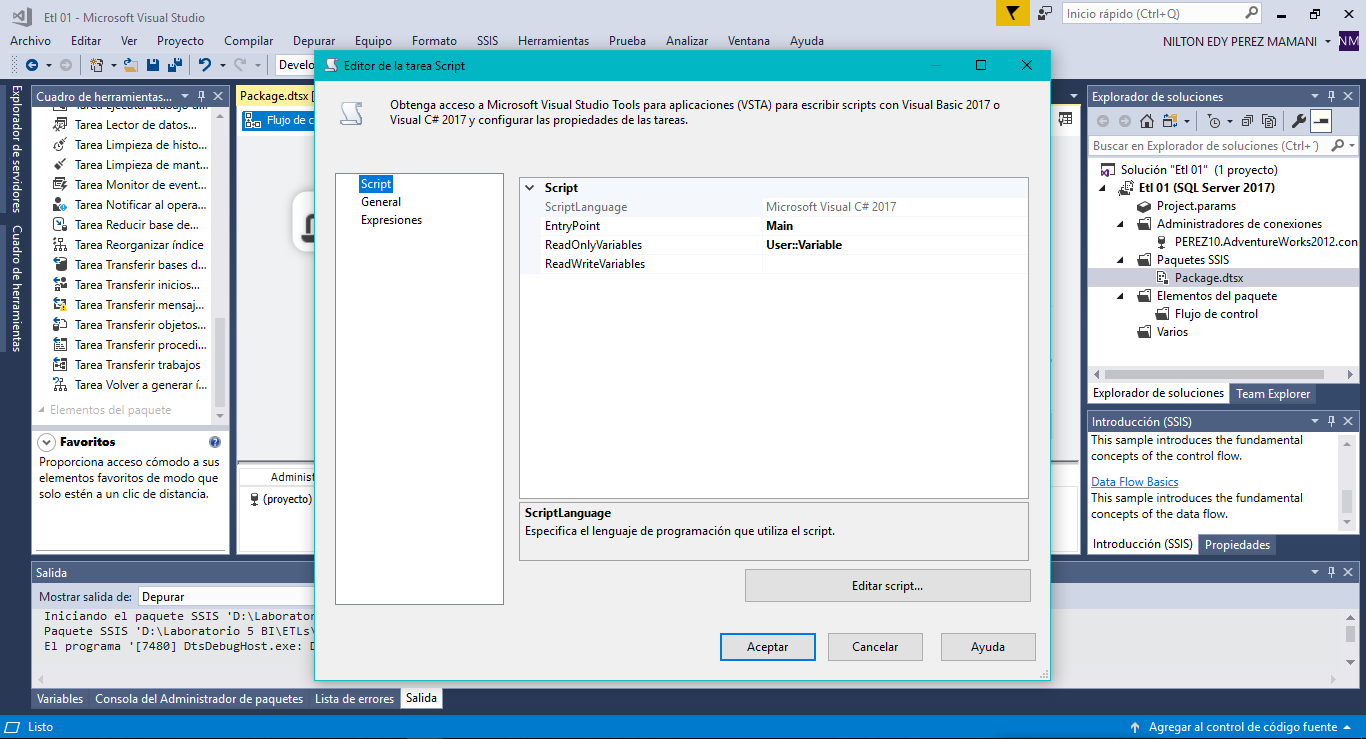
\includegraphics[width=15cm]{./Imagenes/imagen21}
\end{center}
\begin{center}
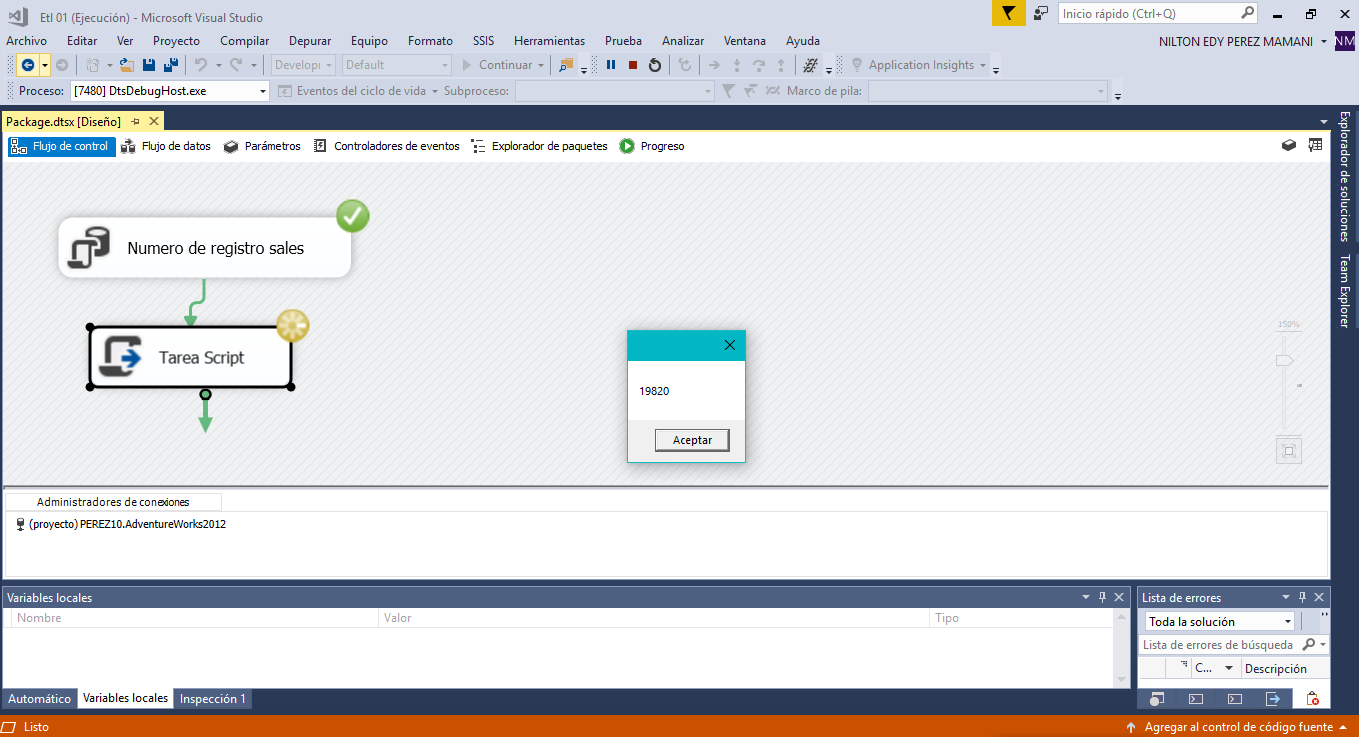
\includegraphics[width=15cm]{./Imagenes/imagen22}
\end{center}
\begin{center}
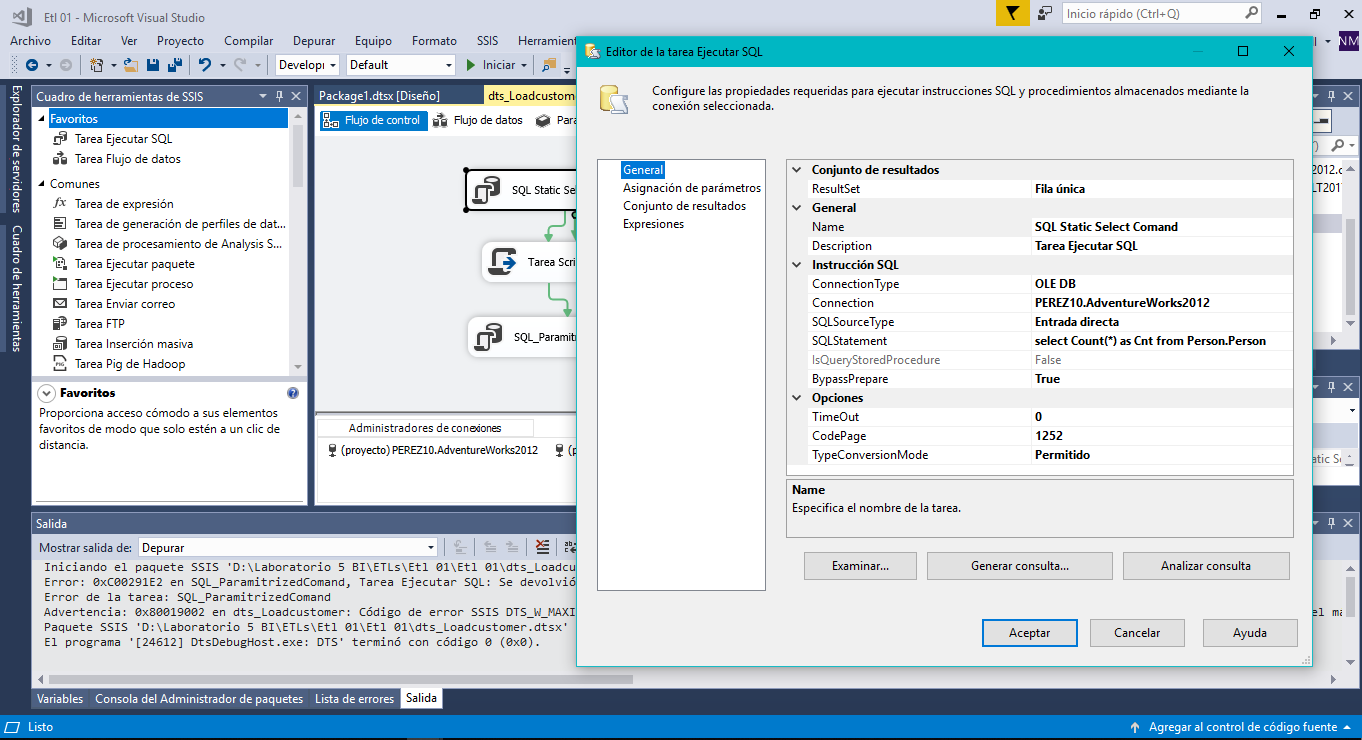
\includegraphics[width=15cm]{./Imagenes/imagen23}
\end{center}
\begin{center}
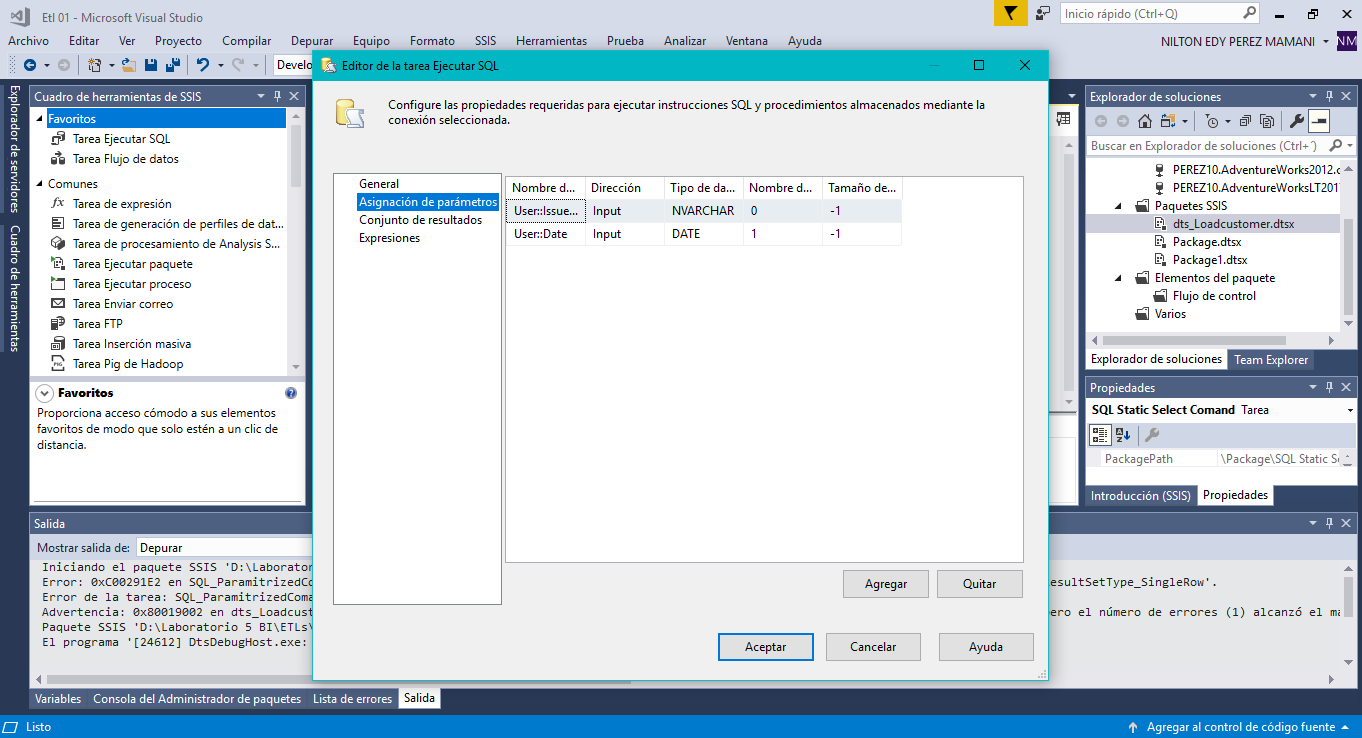
\includegraphics[width=15cm]{./Imagenes/imagen24}
\end{center}
\begin{center}
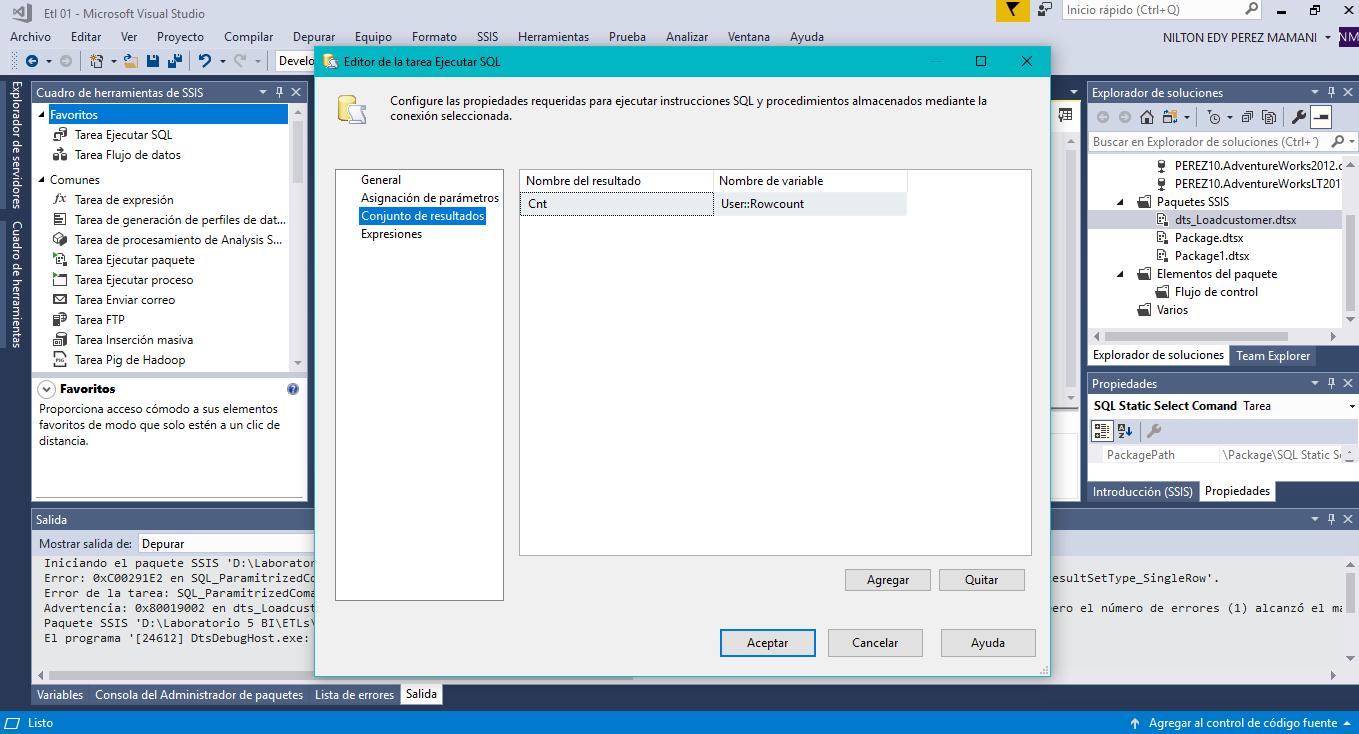
\includegraphics[width=15cm]{./Imagenes/imagen25}
\end{center}
\begin{center}
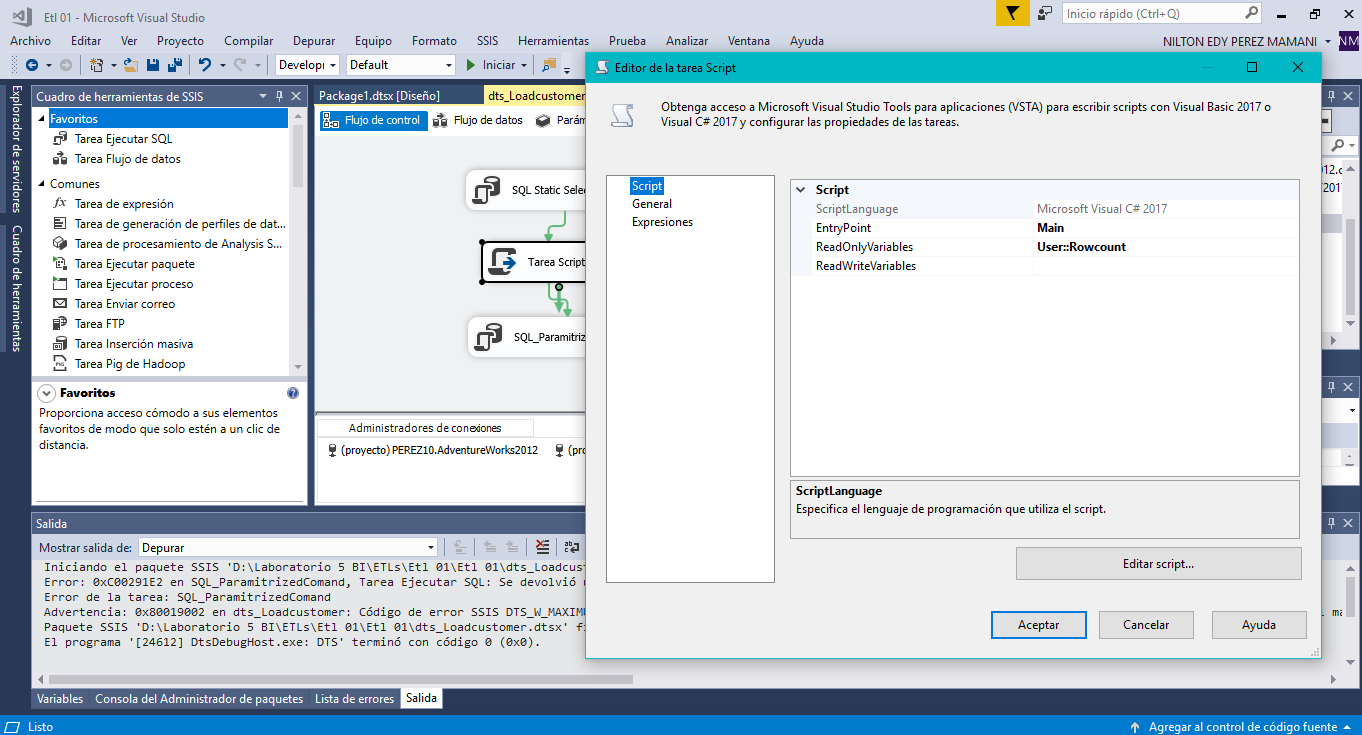
\includegraphics[width=15cm]{./Imagenes/imagen26}
\end{center}
\begin{center}
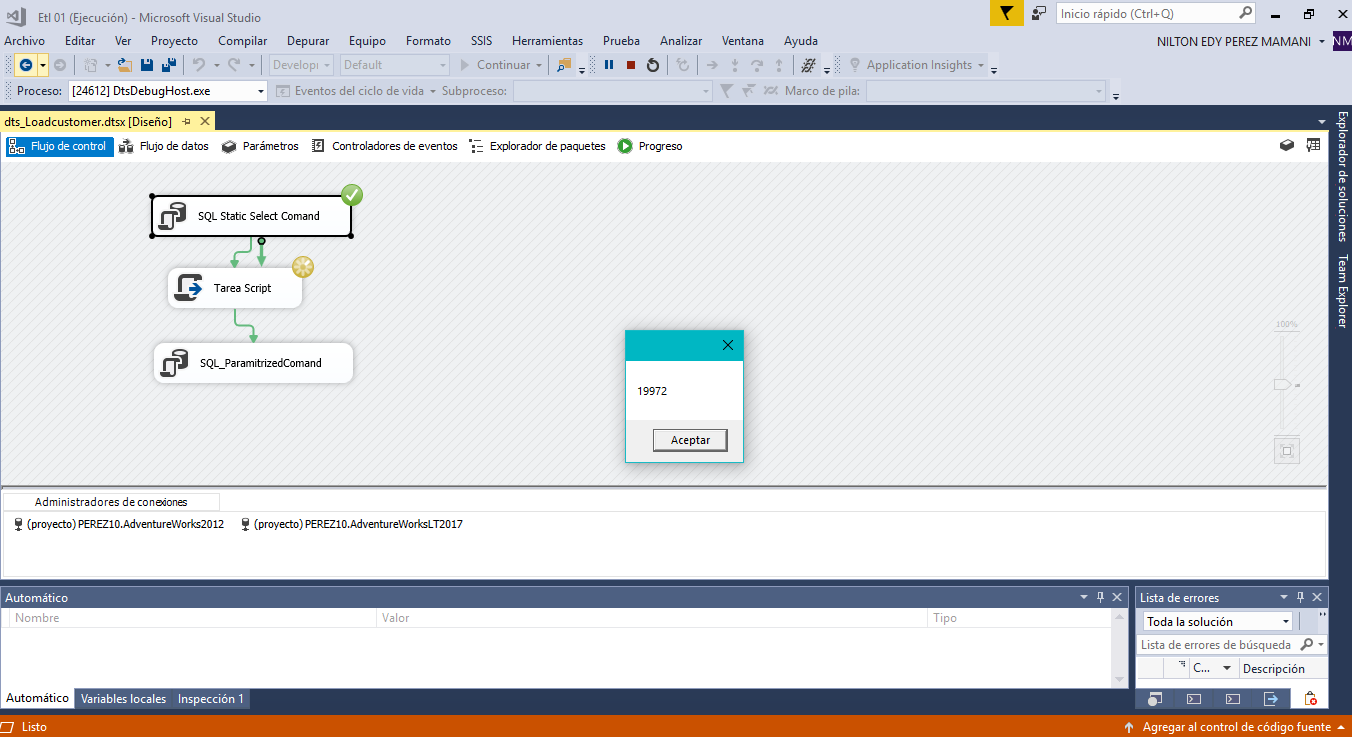
\includegraphics[width=15cm]{./Imagenes/imagen27}
\end{center}
}



% Bibliografía.
%-----------------------------------------------------------------
\begin{thebibliography}{99}

\bibitem{Cd94} Autor, \emph{Título}, Revista/Editor, (año)

\end{thebibliography}

\end{document}


\end{document}
